%%%%%%%%%%%%%%%%%%%%%%%%%%%%%%%%%%%%%%%%%%%%%%%
\chapter{Generalized combination Network} \label{chap:general_network}
%%%%%%%%%%%%%%%%%%%%%%%%%%%%%%%%%%%%%%%%%%%%%%%

\section{Description \label{sec:Description_GCN}}

A generalized combination network $(\epsilon,\ell)-\mathcal{N}_{h,r,s}$
consists of 3 components over 3 layers from top to bottom: ``Source''
in the first layer, ``Intermediate Nodes'' in the middle layer,
and ``Receiver'' in the third layer. Because ``Source'' and ``Receiver''
have their own names without previous confusion of a source node or
a destination node, we replace ``Intermedate Nodes'' by ``Nodes''
from this section. The network has a source with $h$ messages, $r$
nodes, and $\left(\begin{array}{c}
r\\
\alpha
\end{array}\right)$ receivers, which form a single source multicast network modeled as
a finite directed acyclic multigraph \cite{Li:2003}. The source connects
to each node by $\ell$ parallel links and each node also connects
to a receiver by $\ell$ parallel links, which are respectively called
a node's incoming and outgoing links. Each receiver is connected by
$s$ links in total, specifically $\alpha l$ links from $\alpha$
nodes and $\epsilon$ direct links from the source, i.e. $s=\alpha\ell+\epsilon$.
The combination network in \cite{Riis:2006} is the $(0,1)-\mathcal{N}_{h,r,s}$
network and the $(1,1)-\mathcal{N}_{h,r,s}$ network is called One-Direct
Link Combination Network. Theorem 1 shows our interest of relations
between the parameters $h,\alpha,\epsilon$ and $\ell$. Following
to Theorem \ref{nw_parameters}, we are interested in networks parameters
satisfying this condition: $\ell+\epsilon+1\leq h\leq\alpha\ell+\epsilon$.
\begin{figure}[H]
\caption{The generalized network $(\epsilon,\ell)-\mathcal{N}_{h,r,s}$\label{fig:The-generalized-network}}

\centering{}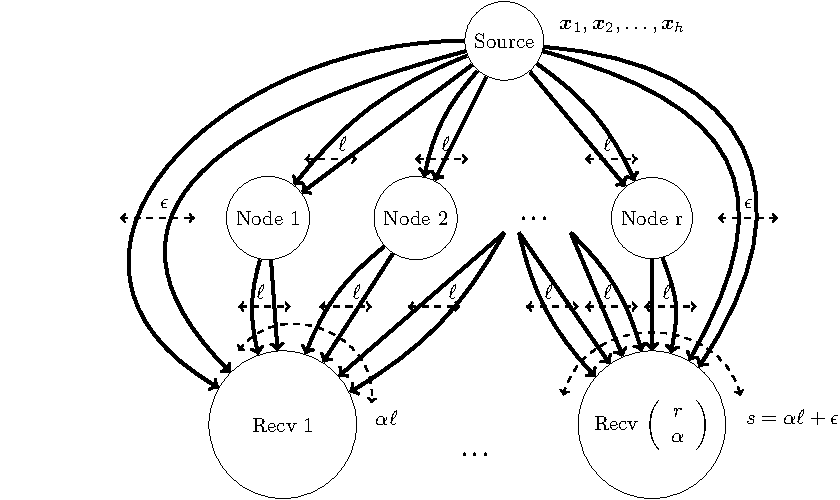
\includegraphics[width=0.5\paperwidth]{E:/Documents/TUM/THESIS/thesisCOD_Ha/figures/generalized_combination_nw}
\end{figure}

\begin{thm}[\cite{Wachter-Zeh:2018}]
\label{nw_parameters}The $(\epsilon,\ell)-\mathcal{N}_{h,r,s}$
network has a trivial solution if $\ell+\epsilon\geq h$, and it has
no solution if $\alpha\ell+\epsilon<h$.

Proof: Following to the network coding max-flow min-cut theorem for
multicast networks, the maximum number of messages from the source
to each receiver is equal to the smallest min-cut between the source
and any receiver. For our considered network, $s$ links have to be
deleted to disconnect the source from the receiver, which implies
that the min-cut between the source and each receiver is at least
$s$. Hence, $h\leq s\Leftrightarrow h\leq\alpha\ell+\epsilon$ $\Square$

There exist at least $\ell+\epsilon$ disjoint links connected to
each receiver. If $\ell+\epsilon\geq h$, each receiver can always
reconstruct its requested messages on its links. Then we only need
to do routing to select paths for the network. $\Square$
\end{thm}
\begin{table}[H]
\caption{Parameters of network coding \label{tab:Parameters-of-network}}

\centering{}%
\begin{tabular}{c|>{\centering}p{0.48\paperwidth}}
$h$ & The number of source messages\tabularnewline
\hline 
$r$ & The number of nodes in the middle layer\tabularnewline
\hline 
$\left(\begin{array}{c}
r\\
\alpha
\end{array}\right)$ & The number of receivers\tabularnewline
\hline 
$\ell$ & The source connects to each node by $\ell$ parallel links, and each
node also connects to one receiver by $\ell$ parallel links\tabularnewline
\hline 
$\alpha$ & A receiver is connected by any $\alpha$ nodes in the middle layer\tabularnewline
\hline 
$\epsilon$ & The source additionally connects to each receiver by $\epsilon$ direct
parallel links\tabularnewline
\hline 
$s$ & Each receiver is connected by $s$ links in total, with $s=\alpha\ell+\epsilon$.\tabularnewline
\end{tabular}
\end{table}


\section{Network Coding for This Network \label{sec:Network-Coding-for-GCN}}

We start describing a difference of a source message used in scalar
network coding and vector network coding. Then we find a condition
for an existence of a scalar solution and a vector solution respectively.
For the $(\epsilon,\ell)-\mathcal{N}_{h,r,s}$ network, the \textit{local}
and \textit{global} coding vectors are the same, because the nodes
are simplified to forward their received packets and only the source
has its functions on its messages.

\subsection{Scalar network coding \label{subsec:Scalar-network-coding}}

A message or a packet is equivalent to a symbol over $\ensuremath{\mathbb{F}}_{q_{\mathrm{s}}}$.
As a network of the multicast model, all receivers request the same
$h$ symbols at the same time \cite{Trautmann:2013}. A transmission
of $h$ data units is a 1-dimentional subspace of $\ensuremath{\mathbb{F}}_{q_{\mathrm{s}}}^{h}$.
Each receiver therefore must obtain a subspace of $\ensuremath{\mathbb{F}}_{q_{\mathrm{s}}}^{h}$,
whose dimension is at least $h$, to be able to reconstruct the packet.
Through $\epsilon$ direct links connected from the source to a receiver,
the source can provide any required $\epsilon$ 1-dimensional subspaces
of $\ensuremath{\mathbb{F}}_{q_{\mathrm{s}}}^{h}$ for the corresponding
receiver. Each receiver can accordingly reconstruct the packet if
and only if the linear span of $\alpha$ $\ell$-dimensional subspaces
of $\ensuremath{\mathbb{F}}_{q_{\mathrm{s}}}^{h}$ from the nodes
is at least of dimension $h-\epsilon$. When this necessary condition
is satisfied, the network is said to have a \textit{solution} or to
be \textit{solvable}.
\begin{thm}[\cite{Riis:2006}]
 The $(0,1)-\mathcal{N}_{h,r,s}$ network has a solution if and only
if there exists an $\left(r,\left|\ensuremath{\mathbb{F}}_{q_{\mathrm{s}}}\right|h,r-\alpha+1\right)$
$\left|\ensuremath{\mathbb{F}}_{q_{\mathrm{s}}}\right|$-ary error
correcting code. 
\end{thm}
%
\begin{thm}[\cite{Zhang:2019}]
 The $(\epsilon,\ell)-\mathcal{N}_{h,r,s=\alpha l+\epsilon}$network
is solvable over $\ensuremath{\mathbb{F}}_{q}$ if and only if there
exists an $\alpha-\left(h,\ell,h-\ell-\epsilon\right)_{q}^{c}$ code
with $r$ codewords. \label{theo:scalar_sol_exist}
\end{thm}

\subsection{Vector network coding \label{subsec:Vector-network-coding}}

In vector network coding, a message or a packet is a vector of length
$t$ over $\ensuremath{\mathbb{F}}_{q}$. A vector solution is therefore
over field size $q$ and dimension $t$. Such a vector solution has
the same alphabet size as a scalar solution of field size $q^{t}$,
and we denote $q_{v}=q^{t}$. A mapping from the scalar solution of
field size $q^{t}$ to an equivalent vector solution is represented
in Example \ref{ex:scalar_vector_mapping}. Similarly with the scalar
\textit{linear} coding solution, each receiver can reconstruct its
requested packet if and only if any $\alpha$ $\left(\ell t\right)$-dimensional
subspaces span a subspace of dimension at least $\left(h-\epsilon\right)t$.
\begin{thm}[\cite{Zhang:2019}]
 A vector solution for the $(\epsilon,\ell)-\mathcal{N}_{h,r,s}$
network exists if and only if there exists $\mathcal{G}_{q}\left(ht,\ell t\right)$
such that any $\alpha$ subspaces of the set span a subspace of dimension
at least $\left(h-\epsilon\right)t$. 
\end{thm}
%
\begin{thm}[\cite{Zhang:2019}]
 The $(\epsilon,\ell)-\mathcal{N}_{h,r,s=\alpha\ell+\epsilon}$network
is solvable with vectors of length $t$ over $\ensuremath{\mathbb{F}}_{q}$
if and only if there exists an $\alpha-\left(ht,\ell t,ht-\ell t-\epsilon t\right)_{q}^{c}$
code with $r$ codewords. 
\end{thm}
\begin{cor}
The $\alpha-\left(n=ht,n-k=ht-\ell t,\lambda=ht-\ell t-\epsilon t\right)_{q}^{m}$
code formed from the dual subspaces of the $\alpha-\left(n=ht,k=\ell t,\lambda=ht-\ell t-\epsilon t\right)_{q}^{c}$
code yields the upper bound of $\mathcal{A}_{q}\left(n=ht,n-k=ht-\ell t,\alpha;\lambda\right)$
as maximum number of nodes for a vector network coding of the $(\epsilon,\ell)-\mathcal{N}_{h,r,s}$
network. \label{cor:dual_subspaces}
\end{cor}
\begin{example}
\label{ex:scalar_vector_mapping} 

Given $h=3,q=2,t=2$, we consider the extension field $\ensuremath{\mathbb{F}}_{q^{t}=2^{2}}$.
This example shows how mapping messages from scalar coding to vector
coding.
\end{example}
\begin{figure}[H]
\caption{The mapping of scalar solution over $\ensuremath{\mathbb{F}}_{q_{\mathrm{s}}=q^{t}}$
to the equivalent vector solution\label{fig:x_mapping}}

\centering{}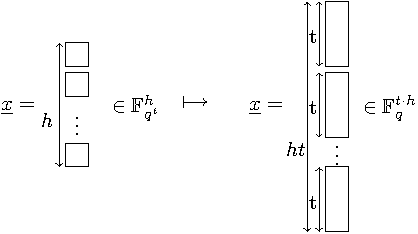
\includegraphics[width=0.3\paperwidth]{E:/Documents/TUM/THESIS/thesisCOD_Ha/figures/x_mapping}
\end{figure}

We use the table of the extension field $\ensuremath{\mathbb{F}}_{2^{2}}$
with the primitive polynomial $f(x)=x^{2}+x+1$:
\begin{center}
\begin{tabular}{|c|c|c|}
\hline 
power of $\alpha$ & polynomial & binary vector\tabularnewline
\hline 
- & 0 & 00\tabularnewline
\hline 
$\alpha^{0}$ & 1 & 01\tabularnewline
\hline 
$\alpha^{1}$ & $\alpha$ & 10\tabularnewline
\hline 
$\alpha^{2}$ & $\alpha+1$ & 11\tabularnewline
\hline 
\end{tabular}
\par\end{center}

For scalar coding, the messages are $x_{1},\ldots,x_{h=3}\in\ensuremath{\mathbb{F}}_{2^{2}}$
, and for vector coding the messages are $\boldsymbol{x}_{1},\ldots,\boldsymbol{x}_{h=3}\in\ensuremath{\mathbb{F}}_{2}^{2}$.
From the polynomial column, let's choose arbitrarily a scalar vector
$\boldsymbol{x}_{scalar}=(x_{1},x_{2},x_{3})=(1,\alpha,\alpha+1)$.
Then, we map it to $\boldsymbol{x}_{vector}=(\boldsymbol{x}_{1},\boldsymbol{x}_{2},\boldsymbol{x}_{3})$
by using the binary vector column as following:

\[
\left[\begin{array}{c}
x_{1}=1\\
x_{2}=\alpha\\
x_{3}=\alpha+1
\end{array}\right]\mapsto\left[\begin{array}{c}
\left(\begin{array}{c}
1\\
0
\end{array}\right)\\
\left(\begin{array}{c}
0\\
1
\end{array}\right)\\
\left(\begin{array}{c}
1\\
1
\end{array}\right)
\end{array}\right],
\]

where we use the following rule for mapping $x_{i}$ individually:
$a_{0}\cdot\alpha^{0}+a_{1}\cdot\alpha^{1}+\ldots+a_{t-1}\cdot\alpha^{t-1}\mapsto\left(\begin{array}{c}
a_{0}\\
a_{1}\\
\vdots\\
a_{t-1}
\end{array}\right)$.

\section{Instances of Generalized Combination Network}

The subsection lists all instances of the $(\epsilon,\ell)-\mathcal{N}_{h,r,s}$
network used by Etzion and Wachter-Zeh in \cite{Wachter-Zeh:2018}
to derive bounds on the corresponding network's gaps between scalar
and vector network coding. They cover small and large values of the
pair $(\epsilon,\ell)$, i.e. $(\epsilon=0,\ell=1)$, $(\epsilon=1,\ell)$,
$(\epsilon,\ell=1)$ and $(\epsilon=l-1,\ell)$. In Section \ref{sec:e1l1_nw},
we study another interesting case $(\epsilon=1,\ell=1)$.

\subsection{The $(\ell-1)$-Direct Links and $\ell$-Parallel Links $\mathcal{N}_{h=2l,r,s=3l-1}$
Network}

This network family is denoted by $\left(\ell-1,\ell\geq2\right)-\mathcal{N}_{2\ell,r,3\ell-1}$.
This family contains the largest number of direct links from the source
to the receivers among all families of GCN. Its vector solution can
be provided by an $\mathcal{MRD}\left[\ell t\times\ell t,t\right]_{q}$
code for any $r_{vector}\leq q^{\ell\left(\ell-1\right)t^{2}+\ell t}$.
There is a scalar solution for this network, if and ony if $r_{scalar}\leq\left[\begin{array}{c}
2\ell\\
\ell
\end{array}\right]_{q_{s}}<4_{q_{s}}^{\ell^{2}}$. Therefore, the gap tends to $q^{t^{2}+\mathcal{O}\left(t\right)}$
for large $\ell$.
\begin{figure}[H]
\caption{The $\left(1,2\right)-\mathcal{N}_{4,r,5}$ network as an example
of the $\left(\ell-1,\ell\right)-\mathcal{N}_{2\ell,r,3\ell-1}$ \label{fig:network_l1e2h4rs5}}

\centering{}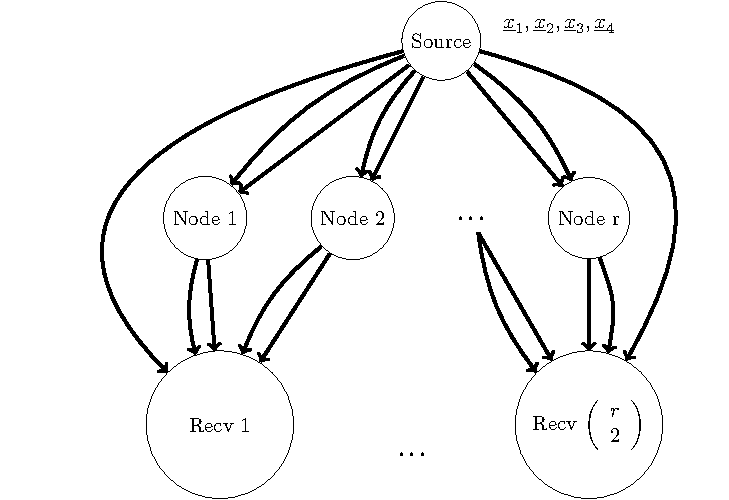
\includegraphics[width=0.4\paperwidth]{E:/Documents/TUM/THESIS/thesisCOD_Ha/figures/nw_e1_l2_h4_r_s5}
\end{figure}


\subsection{The 1-Direct Link and $\ell$-Parallel Links $\mathcal{N}_{h=2\ell,r,s=2\ell+1}$
Network}

We denote this network family by $(1,\ell\geq2)-\mathcal{N}_{2\ell,r,2\ell+1}$.
This network family is the family with the smallest number of direct
links, such that Etzion and Wachter-Zeh's vector solution outperforms
the optimal scalar solution, i.e. an vector solution outperforming
the optimal scalar has not yet been found for the network $(0,\ell\geq2)-\mathcal{N}_{h,r,s}$.
When $\ell\geq2$ or $h\geq4$, they proved that this network has
a vector solution based on an $\mathcal{MRD}\left[\ell t\times\ell t,(\ell-1)t\right]_{q}$
code when $r=q^{\ell t\left(t+1\right)},$and scalar solutions only
if $q_{s}>q^{t^{2}/2}$. Therefore, this network has a gap tending
to $q^{t^{2}/2+\mathcal{O}\left(t\right)}$ with a vector solution
.

\begin{figure}[H]
\caption{The $\left(\ell-1,\ell\right)-\mathcal{N}_{2\ell,r,3\ell-1}$ network
\label{fig:network_special2}}

\centering{}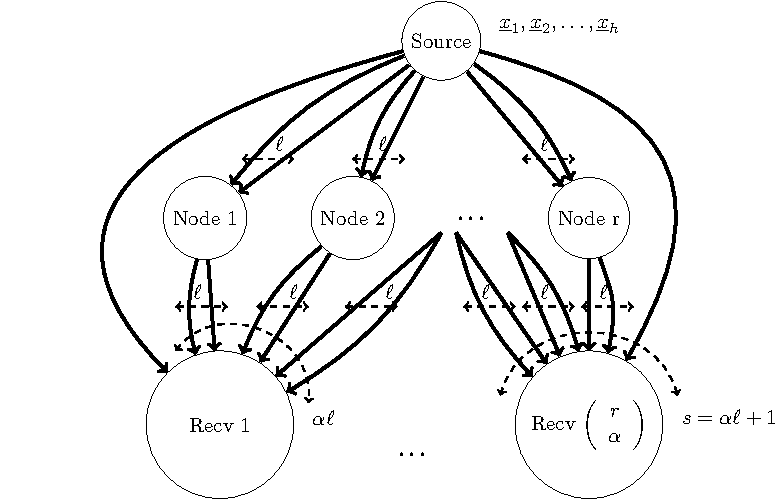
\includegraphics[width=0.45\paperwidth]{E:/Documents/TUM/THESIS/thesisCOD_Ha/figures/nw_special2}
\end{figure}


\subsection{The $\epsilon$-Direct Links $\mathcal{N}_{h,r,s}$}

This network family is denoted by $\left(\epsilon\geq1,\ell=1\right)-\mathcal{N}_{h,r,s}$
and is the main focus of this thesis, because it motivates some interesting
questions on a classic coding problem and on a new type of subspace
code problem. Furthermore, there is no gap size is known for this
network in previous studies. In Section \ref{sec:Network_e1l1h3rs4},
we show that there exists vector solutions generating the gaps $g=q^{t^{2}/4+\mathcal{O}(t)}$
and $g=q^{\frac{\alpha-h+1}{\left(\alpha-1\right)\left(\alpha-h+2\right)\left(h-2\right)}t^{2}+\mathcal{O}(t)}$
respectively for the $\left(1,1\right)-\mathcal{N}_{3,r,4}$ network
and the $\left(1,1\right)-\mathcal{N}_{h,r,s}$ network. 

\begin{figure}[H]
\caption{The $\left(\epsilon\protect\geq1,\ell=1\right)-\mathcal{N}_{h,r,s}$
network \label{fig:network_special3}}

\centering{}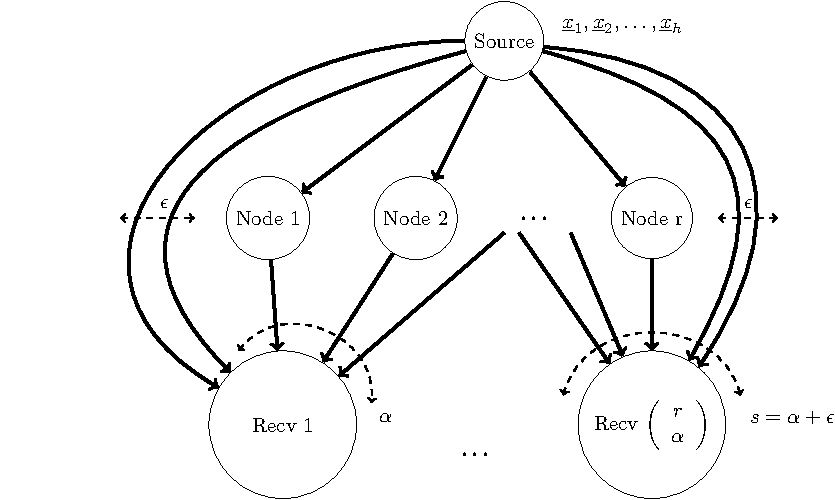
\includegraphics[width=0.45\paperwidth]{E:/Documents/TUM/THESIS/thesisCOD_Ha/figures/nw_special3}
\end{figure}


\subsection{The $\left(\epsilon=0,\ell=1\right)-\mathcal{N}_{h,r,s}$ Combination
Network}

Since the scalar solution for the combination network uses an $MDS$
code, a vector solution based on subspace codes must go beyond the
$MDS$ bound, i.e. Singleton bound $d\leq n-k+1$, to outperform the
scalar one. In paper \cite[Sec. IV-A, Sec. IX-1,2]{Wachter-Zeh:2018},
it is proved that vector solutions based on subspace codes cannot
outperform optimal scalar linear solutions for some combination networks,
e.g. $\mathcal{N}_{2,r,2}$, and they conjecture it for all $h$. 

\begin{figure}[H]
\caption{The $\left(\epsilon=0,\ell=1\right)-\mathcal{N}_{h,r,s}$ combination
network \label{fig:network_special4}}

\centering{}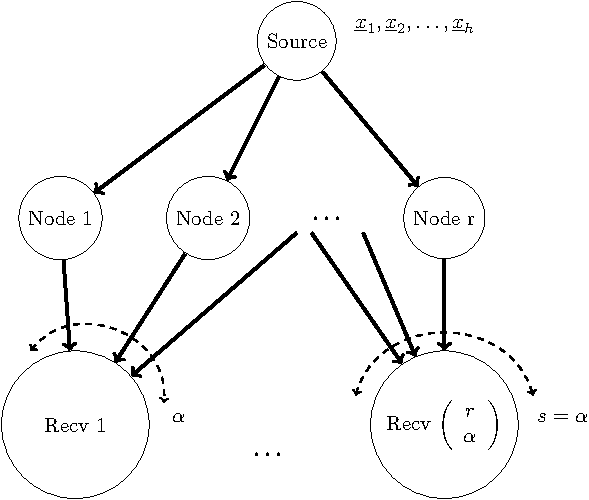
\includegraphics[width=0.4\paperwidth]{E:/Documents/TUM/THESIS/thesisCOD_Ha/figures/nw_special4_combination}
\end{figure}


\subsection{The Largest Possible Gap between $q_{v}$ and $q_{s}$ in Previous
Studies}

Etzion and Wachter-Zeh considered 2 cases separately $h\leq2\ell,\epsilon\neq0$
and $h\geq2\ell,\epsilon\neq h-2\ell$

\subsubsection{\uline{\mbox{$h\protect\leq2\ell$} and \mbox{$\epsilon\protect\neq0$}}}

For this network, the number of direct links is at least 1, i.e. $\epsilon\geq1$,
and the number of parallel links is less than half of the number of
source messages, i.e. $\ell\leq\frac{h}{2}$.

\paragraph{h is even}

The above $\left(\ell-1,l\right)-\mathcal{N}_{2\ell,r,3\ell-1}$ network
achieves the largest gap $q_{\mathrm{s}}=q^{(h-2)t^{2}/h+\mathcal{O}(t)}$.

\paragraph{h is odd}

The $\left(\ell-2,\ell\right)-\mathcal{N}_{2\ell-1,r,3\ell-2}$ network
achieves the largest gap $q_{\mathrm{s}}=q^{\left(h-3\right)t^{2}/\left(h-1\right)+\mathcal{O}(t)}$

\subsubsection{\uline{\mbox{$h\protect\geq2\ell$} and \mbox{$\epsilon\protect\neq h-2\ell$}}}

\paragraph{h is even}

The same above $\left(\ell-1,\ell\right)-\mathcal{N}_{2\ell,r,3\ell-1}$
network achieves the largest gap $q_{s}=q^{(h-2)t^{2}/h+\mathcal{O}(t)}$.

\paragraph{h is odd}

The $\left(\ell-1,\ell\right)-\mathcal{N}_{2\ell+1,r,3\ell-1}$ network
achieves the largest gap $q_{\mathrm{s}}=q^{(h-3)t^{2}/\left(h-1\right)+\mathcal{O}(t)}$.
\begin{rem}
The achieved gap is $q^{(h-2)t^{2}/h+\mathcal{O}(t)}$ for any $q\geq2$
and any even $h\geq4$. If $h\geq5$ is odd, then the achieved gap
of the alphabet size is $q^{(h-3)t^{2}/\left(h-1\right)+\mathcal{O}(t)}$
\cite{Wachter-Zeh:2018}.
\end{rem}
We are summarizing the instances of GCN with their bounds on gap found
in \cite{Wachter-Zeh:2018} and list our findings in this study.

\begin{table}

\caption{New gap found in this study}

\begin{centering}
\begin{tabular}{|>{\centering}p{0.15\paperwidth}|>{\centering}p{0.1\paperwidth}|>{\centering}p{0.2\paperwidth}|}
\hline 
\centering{}Network & \centering{}Gap Bounds for a specific vector solution \cite{Wachter-Zeh:2018} & \centering{}This study proves an existence of these gaps\tabularnewline
\hline 
\hline 
\centering{}$\left(\epsilon=0,\ell=1\right)-\mathcal{N}_{h,r,s}$ & \centering{}N/A & \centering{}N/A\tabularnewline
\hline 
\centering{}$\left(\epsilon\geq1,\ell=1\right)-\mathcal{N}_{h,r,s}$ & \centering{}Unknown & \centering{}$q^{\frac{\alpha-h+1}{\left(\alpha-1\right)\left(\alpha-h+2\right)\left(h-2\right)}t^{2}+\mathcal{O}(t)}$
({*})\tabularnewline
\hline 
\begin{centering}
$(\epsilon=1,\ell\geq2)-$
\par\end{centering}
$\mathcal{N}_{h=2\ell,r,s=2\ell+1}$ & \centering{}$q^{t^{2}/2+\mathcal{O}\left(t\right)}$ & \centering{}$q^{t^{2}/l+\mathcal{O}\left(t\right)}$\tabularnewline
\hline 
\begin{centering}
$\left(\epsilon=\ell-1,\ell\right)-$
\par\end{centering}
$\mathcal{N}_{h=2\ell,r,s=3\ell-1}$ & \centering{}$q^{t^{2}/2+\mathcal{O}\left(t\right)}$ & \centering{}N/A\tabularnewline
\hline 
\end{tabular}
\par\end{centering}
\begin{centering}
({*}): We only consider the $\left(\epsilon=1,\ell=1\right)-\mathcal{N}_{h,r,s}$
network.
\par\end{centering}
\end{table}

Some of them has global coding vectors as square matrices, so the
decoding base easily by inversing such global coding vectors to get
each receiver's requested messages. However, we do not go into details
of decoding methods in this study.

\clearpage